% Documento principal. Overleaf: selecionar main.tex e compilar com XeLaTeX.
% Para revisão cega, selecionar submissao_cega.tex.
\documentclass[12pt,a4paper]{article}
\usepackage[T1]{fontenc}
\usepackage[utf8]{inputenc}
\usepackage[spanish,english,brazil]{babel}
\usepackage{newtxtext,newtxmath}
\usepackage[margin=2.5cm]{geometry}
\usepackage{graphicx,booktabs,tabularx,array,amsmath}
\usepackage{setspace,indentfirst,microtype}
\usepackage[round,authoryear,semicolon,sort]{natbib}
\usepackage{caption,placeins}
\usepackage{xurl}
\usepackage[hidelinks,unicode]{hyperref}
\hypersetup{pdfauthor={},pdftitle={Modelagem dos manguezais da costa macrotidal da Amazônia sob cenários de elevação do nível do mar até o final do século XXI}}
\setlength{\parindent}{1.25cm}
\setlength{\parskip}{0pt}
\setstretch{1.15}
\setlength{\emergencystretch}{2em}
\captionsetup{font=small,labelfont=bf,labelsep=period,justification=justified,singlelinecheck=false}
\setlength{\bibsep}{0.7\baselineskip}
\renewcommand{\bibsection}{\section*{Referências}}
\renewcommand{\bibfont}{\small\singlespacing\raggedright}
\newcommand{\fonte}[1]{\par\smallskip{\footnotesize\raggedright #1\par}}
\newcommand{\tituloPT}{Modelagem dos manguezais da costa macrotidal da Amazônia sob cenários de elevação do nível do mar até o final do século XXI}
\begin{document}
\begin{center}
{\Large\bfseries\tituloPT\par}
\vspace{0.7em}
\ifdefined\VersaoCega\else
Felipe Martins Sousa; Denilson da Silva Bezerra;\\
Sergio Souza Costa; Ricardo Luvizotto Santos\\[0.35em]
{\small Universidade Federal do Maranhão\\
Programa de Pós-Graduação em Ciência e Tecnologia Ambiental, Brasil}
\fi
\end{center}

\section*{Resumo}
A elevação do nível do mar afeta a permanência e a expansão dos manguezais, condicionadas pela sedimentação, pelo relevo e pelo espaço para migração. Este estudo simula a dinâmica dos manguezais da costa de macromaré entre 2025 e 2100, sob três cenários de elevação. \ifdefined\VersaoCega Aplica-se um modelo baseado em autômatos celulares, com cobertura do MapBiomas Coleção 11, terreno do ANADEM e trajetórias regionais do IPCC AR6 para SSP1-2.6, SSP2-4.5 e SSP5-8.5.\else Aplica-se o BR-MANGUE Studio, modelo baseado em autômatos celulares, com cobertura do MapBiomas Coleção 11, terreno do ANADEM e trajetórias regionais do IPCC AR6 para SSP1-2.6, SSP2-4.5 e SSP5-8.5.\fi\space As simulações anuais usam células de 30 m, acreção sedimentar fixa de 2,4 mm ano$^{-1}$ e atraso funcional de três anos para que células migradas passem a atuar como fontes de propágulos. A área simulável contém 6.758,9 km$^2$ de manguezais em 2025. Em 2100, a extensão simulada alcança 6.003,2, 5.881,8 e 5.697,4 km$^2$, reduções líquidas de 11,18\%, 12,98\% e 15,70\%, respectivamente. A migração acrescenta de 579,0 a 666,0 km$^2$ e não compensa a inundação da cobertura inicial. Florestas alagáveis correspondem a aproximadamente 58,4\% da área convertida em mangue migrado. Os resultados são condicionados pelas trajetórias e regras do modelo; áreas naturais adjacentes favorecem a acomodação espacial dos manguezais.

\noindent\textbf{Palavras-chave:} Manguezais; Amazônia costeira; Autômatos celulares; Elevação do nível do mar; Migração continental.

\section*{Modeling mangroves on the Amazon macrotidal coast under sea-level rise scenarios through the end of the 21st century}
\begin{otherlanguage}{english}
\noindent\textbf{Abstract.} Sea-level rise modifies the conditions for mangrove persistence and expansion, whose response depends on sedimentation, topography and the availability of migration space. This study simulates the spatial dynamics of mangroves on the Amazon macrotidal coast between 2025 and 2100 under three sea-level rise scenarios. \ifdefined\VersaoCega A model based on cellular automata is applied using MapBiomas Collection 11 land cover, ANADEM terrain elevation and regional IPCC AR6 trajectories for SSP1-2.6, SSP2-4.5 and SSP5-8.5.\else BR-MANGUE Studio, a model based on cellular automata, is applied using MapBiomas Collection 11 land cover, ANADEM terrain elevation and regional IPCC AR6 trajectories for SSP1-2.6, SSP2-4.5 and SSP5-8.5.\fi\space Annual simulations use 30-m cells, a fixed sediment accretion rate of 2.4 mm yr$^{-1}$, and a three-year functional delay before migrated cells can act as propagule sources. The simulated area contains 6,758.9 km$^2$ of mangroves in 2025. By 2100, simulated extent reaches 6,003.2, 5,881.8 and 5,697.4 km$^2$, corresponding to net reductions of 11.18\%, 12.98\% and 15.70\%, respectively. Migration adds between 579.0 and 666.0 km$^2$, insufficient to offset inundation of the initial cover. Floodable forests account for approximately 58.4\% of the area converted to migrated mangrove. The results are conditional on the adopted trajectories and model rules; adjacent natural areas provide space for mangrove migration.

\noindent\textbf{Keywords:} Mangroves; Coastal Amazon; Cellular automata; Sea-level rise; Landward migration.
\end{otherlanguage}

\section*{Modelación de los manglares de la costa macromareal amazónica bajo escenarios de aumento del nivel del mar hasta finales del siglo XXI}
\begin{otherlanguage}{spanish}
\noindent\textbf{Resumen.} La elevación del nivel del mar afecta la permanencia y expansión de los manglares, condicionadas por sedimentación, relieve y espacio disponible para migrar. Este estudio simula la dinámica de los manglares de la costa amazónica macromareal entre 2025 y 2100 bajo tres escenarios. \ifdefined\VersaoCega Se aplica un modelo basado en autómatas celulares con cobertura de MapBiomas Colección 11, elevación de ANADEM y trayectorias regionales del IPCC AR6 para SSP1-2.6, SSP2-4.5 y SSP5-8.5.\else BR-MANGUE Studio, un modelo basado en autómatas celulares, integra cobertura de MapBiomas Colección 11, elevación de ANADEM y trayectorias regionales del IPCC AR6 para SSP1-2.6, SSP2-4.5 y SSP5-8.5.\fi\space Las simulaciones anuales usan celdas de 30 m, acreción sedimentaria fija de 2,4 mm año$^{-1}$ y un atraso funcional de tres años para que las células migradas actúen como fuentes de propágulos. El área simulable contiene 6.758,9 km$^2$ de manglares en 2025. En 2100, la extensión alcanza 6.003,2, 5.881,8 y 5.697,4 km$^2$ (reducciones del 11,18\%, 12,98\% y 15,70\%). La migración añade de 579,0 a 666,0 km$^2$ y no compensa la inundación inicial. Los bosques inundables representan aproximadamente el 58,4\% del área convertida en manglar migrado. Los resultados dependen de las trayectorias y reglas adoptadas; las áreas naturales adyacentes ofrecen espacio para la migración de los manglares.

\noindent\textbf{Palabras clave:} Manglares; Amazonía costera; Autómatas celulares; Aumento del nivel del mar; Migración continental.
\end{otherlanguage}

\section{Introdução}
Os manguezais ocupam a interface entre ambientes terrestres e marinhos e sustentam funções ecológicas relacionadas à produção pesqueira, à proteção costeira e ao armazenamento de carbono \citep{lee2014,kauffman2018}. Sua distribuição acompanha condições de inundação, salinidade e estabilidade do substrato, que se alteram com a elevação do nível relativo do mar. A capacidade de manutenção desses ecossistemas depende da combinação entre ganho de elevação da superfície e deslocamento da vegetação para áreas de acomodação lateral \citep{woodroffe2016}. A elevação projetada do nível do mar ao longo do século XXI amplia essas pressões; as respostas variam com o ganho de elevação da superfície e o espaço para migração, com riscos e limiares distintos entre regiões \citep{fox2021,gilman2008,saintilan2020}.

A relação entre elevação do mar e perda de manguezais apresenta forte dependência do contexto ambiental. Lovelock et al.\ \citeyearpar{lovelock2015} demonstram que o suprimento de sedimentos influencia a capacidade de manutenção da elevação da superfície em manguezais do Indo-Pacífico. Schuerch et al.\ \citeyearpar{schuerch2018} incorporam a acreção e o espaço de acomodação em projeções globais de áreas úmidas costeiras e mostram a importância da migração continental para o balanço de área. Modelos que representam interações entre vegetação, hidrodinâmica e transporte sedimentar também indicam que a resposta depende da configuração costeira e das condições de contorno \citep{xie2022}. Assim, o mesmo aumento do nível do mar pode produzir combinações distintas de permanência, inundação e expansão da vegetação.

Na costa norte do Brasil, a Costa de Manguezais de Macromaré da Amazônia (CMMA) reúne extensas planícies estuarinas entre o Pará e o Maranhão. Souza-Filho \citeyearpar{souzafilho2005} caracteriza seus setores geomorfológicos e estima 7.591,09 km$^2$ de manguezais a partir de imagens de 1999--2000. Na área mapeada por Nascimento Jr. et al.\ \citeyearpar{nascimento2013}, a cobertura aumentou de aproximadamente 6.705 km$^2$ em 1996 para 7.423,6 km$^2$ em 2008: o ganho líquido de 718,6 km$^2$ resultou de 1.931 km$^2$ de expansão e 1.213 km$^2$ de erosão, enquanto 5.493 km$^2$ permaneceram estáveis. Estudos de limites da vegetação e de evolução decadal demonstram a coexistência de expansão e retração em setores amazônicos, associadas às mudanças costeiras e ambientais \citep{cohen2003,cohen2018}. A ocupação humana acrescenta restrições espacialmente desiguais ao uso e à continuidade dos manguezais \citep{hayashi2019}.

A modelagem por autômatos celulares representa processos espaciais por estados discretos e regras locais aplicadas a células vizinhas \citep{engelen1995}. \ifdefined\VersaoCega Um estudo anterior aplicou essa abordagem na Ilha do Maranhão, incorporando a influência de áreas antropizadas \citeyearpar{bezerra2014}.\else Bezerra et al.\ \citeyearpar{bezerra2014} utilizam essa abordagem na Ilha do Maranhão, incorporando a influência de áreas antropizadas.\fi\space Tomaz et al.\ \citeyearpar{tomaz2019} simulam a porção maranhense da CMMA, associada às Reentrâncias Maranhenses, de 2010 a 2100 com taxa constante de 3,18 mm ano$^{-1}$ e identificam compensação de perdas pela migração. Esse antecedente fundamenta aplicações com abrangência ampliada ao Pará e Maranhão, dados atualizados e trajetórias temporais de elevação. As projeções do IPCC AR6 permitem representar diferenças entre cenários de emissões e a evolução dos incrementos anuais, enquanto séries de cobertura e modelos de terreno ampliam a disponibilidade de entradas espacialmente explícitas \citep{garner2021,kopp2023,laipelt2024,mapbiomas2026}.

O estudo simula a dinâmica espacial dos manguezais da CMMA entre 2025 e 2100 sob SSP1-2.6, SSP2-4.5 e SSP5-8.5, integrando MapBiomas Coleção 11, ANADEM e projeções regionais do IPCC AR6 \ifdefined\VersaoCega em um modelo espacial.\else no BR-MANGUE Studio.\fi\space Quantificam-se permanência, inundação, migração e categorias de origem, mantendo os demais parâmetros constantes para comparar as três forçantes. Os resultados podem apoiar a discussão de adaptação climática e conservação de ecossistemas costeiros, em diálogo com as metas 13.1, 13.2, 14.2 e 15.1 dos Objetivos de Desenvolvimento Sustentável e com o eixo Meio Ambiente Valorizado e Resiliente do Plano Maranhão 2050, que prevê estruturar a gestão dos recursos naturais e mitigar impactos das mudanças climáticas \citep{unitednations2015,maranhao2050}.

\section{Materiais e métodos}
\subsection{Área de estudo e bases espaciais}
O recorte operacional abrange a faixa costeira entre a Baía de Marajó, no Pará, e a Baía de Tubarão, no Maranhão (Figura~\ref{fig:localizacao}). A costa estudada reúne baías, ilhas, canais e planícies estuarinas; amplitudes de maré entre 4 e 7,5 m foram reportadas para trechos entre Pará e Maranhão \citep{souzafilho2005,menezes2008}. A vegetação inclui espécies dos gêneros \textit{Rhizophora}, \textit{Avicennia} e \textit{Laguncularia}, cuja composição e estrutura variam entre os setores costeiros \citep{menezes2008}. A estatística oficial da Coleção 11 registra 10.436,29 km$^2$ de manguezais no Brasil em 2025; o recorte deste estudo corresponde a 65,0\% desse total mapeado \citep{mapbiomasareas2026}.

\begin{figure}[htbp]
\centering
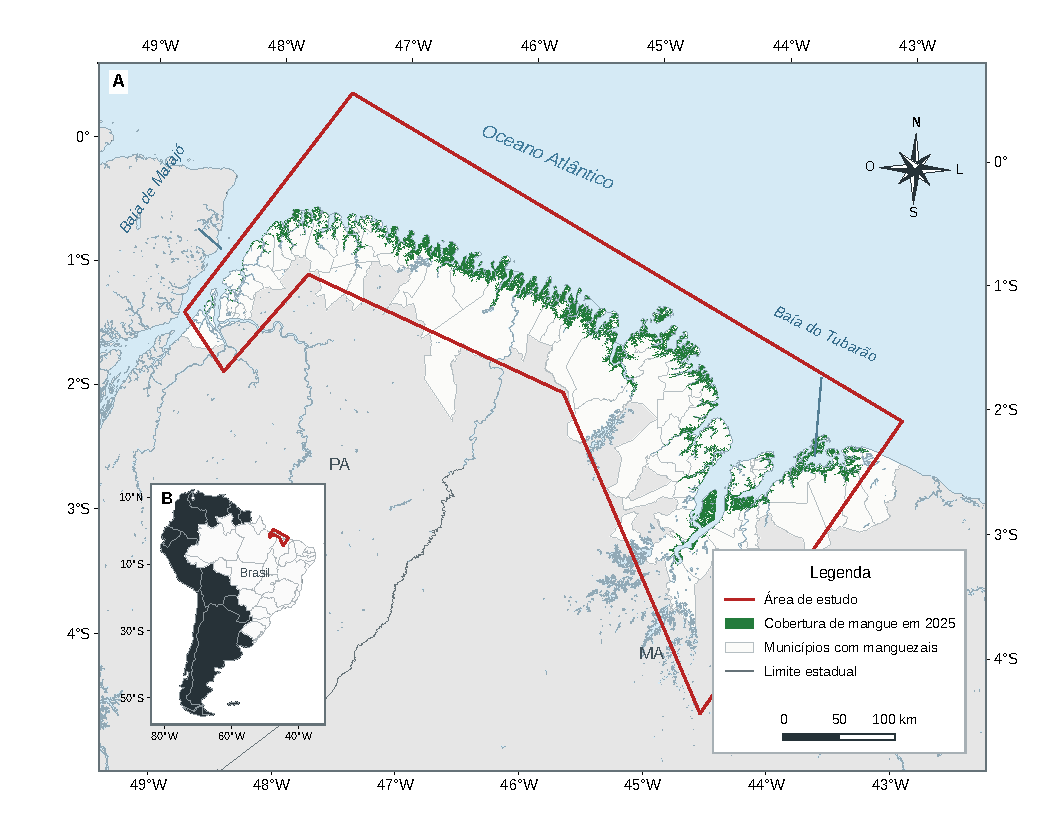
\includegraphics[width=\linewidth]{figuras/figura_1.pdf}
\caption{Localização da área de estudo. (A) Recorte da CMMA, cobertura de mangue em 2025 e municípios com centros de pixels de manguezal no recorte. (B) Localização no Brasil e na América do Sul. A cobertura mapeada inclui áreas sem elevação válida, excluídas da área efetivamente simulada. Projeção do painel A: SIRGAS 2000 / Brazil Albers.}
\label{fig:localizacao}
\fonte{Fontes: MapBiomas Coleção 11; malha municipal IBGE 2025; massas de água IBGE BC250, versão 2025 \citep{ibgebc}; Natural Earth, versão 5.1.1 \citep{naturalearth}. Elaboração a partir das bases citadas.}
\end{figure}

A cobertura da terra provém da Coleção 11 do MapBiomas, com resolução de 30 m e série de 1985--2025 \citep{mapbiomas2026}. A banda de 2025 fornece a condição inicial e preserva todas as categorias presentes no recorte. O produto resulta da classificação de imagens Landsat; a metodologia geral de produção de séries anuais no Brasil é descrita por Souza Jr. et al.\ \citeyearpar{souzajr2020}. Os dados são extraídos no Google Earth Engine \citep{gorelick2017}. A elevação provém do ANADEM v1, modelo de terreno que reduz o efeito da vegetação no Copernicus GLO-30 por aprendizagem de máquina e informações de sensoriamento remoto \citep{laipelt2024}.

As bases são alinhadas a uma grade de 30 $\times$ 30 m em SIRGAS 2000 / Brazil Albers (EPSG:10857), por vizinho mais próximo para cobertura e interpolação bilinear para elevação. A máscara retém centros de pixels internos ao polígono com ambas as entradas válidas. Dos 392.092.180 pixels da grade retangular, 77.061.011 integram o domínio efetivo (69.354,91 km$^2$). A referência vertical do ANADEM permanece EGM2008; a reprojeção horizontal não a modifica \citep{anadem2025}.

O inventário utiliza a Malha Municipal Digital 2025 do IBGE \citep{ibge2025}. Atribui-se cada pixel de manguezal ao polígono que contém seu centro e multiplica-se a contagem por 0,0009 km$^2$. Pixels sem correspondência municipal permanecem em categoria residual. A Planilha Suplementar S1 informa códigos IBGE, municípios e áreas no recorte, com e sem exigência de elevação válida.

\subsection{Modelo, classes e regras de transição}
\ifdefined\VersaoCega Utiliza-se o motor contínuo da versão 1.4.4 de um modelo de autômatos celulares; os dados bibliográficos da implementação são omitidos nesta cópia para avaliação cega \citep{studio2026}. O modelo deriva de uma aplicação anterior na Ilha do Maranhão \citeyearpar{bezerra2014}.\else Utiliza-se o motor contínuo do BR-MANGUE Studio 1.4.4, DOI \url{https://doi.org/10.5281/zenodo.23527116} \citep{studio2026}, derivado da abordagem de Bezerra et al.\ \citeyearpar{bezerra2014}.\fi\space Cada célula contém cobertura, elevação e idade funcional quando migrada. A vizinhança de Moore abrange até oito células válidas adjacentes. Executam-se 75 atualizações anuais, de 2026 a 2100, preservando-se 2025 como referência.

Os 20 códigos MapBiomas são agrupados em manguezal (5), vegetação natural (3, 4, 6, 11, 12 e 50), água (33), área antropizada (9, 15, 21, 24, 25, 30, 31, 35, 39 e 41) e área bloqueada (23 e 32: praia, duna e areal; apicum). Áreas antropizadas e bloqueadas não recebem migração. Estados inundados das classes terrestres e o mangue migrado completam os dez estados possíveis. A correspondência entre códigos de entrada e classes do modelo está no Material Suplementar S1, Seção S2, Tabela S2.

A aptidão do solo é desativada pela ausência de base validada para essa finalidade. A migração em vegetação natural depende de vizinhança e limite altimétrico. O código 33 reúne rios, lagos e oceano, sem separação por salinidade ou conexão mareal.

A implementação arquivada \citep{studio2026} utiliza cópias dos estados, elevações e idades do início do ano para propagar a inundação. Cada célula de água ou inundada com elevação não negativa reparte o incremento anual do nível do mar entre si e seus vizinhos de menor elevação. Esses vizinhos recebem o acréscimo e, quando possuem classe básica com transição disponível, passam ao estado inundado correspondente. A regra e as variáveis estão detalhadas no Material Suplementar S1, Seção S2, Equação S1.

A migração consulta os valores correntes durante a varredura. Manguezais iniciais e células migradas com idade mínima de três anos convertem vizinhos de vegetação natural quando sua elevação é menor ou igual a $T+L_t$, sendo $T$ a referência de maré e $L_t$ a elevação acumulada desde 2025, em metros. A idade da nova célula inicia em zero. Em cada passo anual, o modelo soma 0,0024 m à cota das células com comportamento de mangue; esse incremento corresponde à taxa fixa de acreção sedimentar de 2,4 mm ano$^{-1}$, aplicada como parâmetro uniforme. O estado migrado não apresenta inundação posterior na versão aplicada, tornando sua área cumulativa. As regras são comuns aos três cenários.

\subsection{Trajetórias de elevação do nível do mar}
As forçantes utilizam as projeções regionais do IPCC AR6, versão 20210809, confiança média e percentil 50 \citep{garner2021}. O produto combina expansão térmica, geleiras, mantos de gelo e armazenamento continental de água com padrões regionais e processos de fundo do nível relativo do mar \citep{fox2021,kopp2023}. SSP1-2.6, SSP2-4.5 e SSP5-8.5 representam diferentes trajetórias futuras de emissões.

Selecionam-se nove centros da grade regular nativa internos ao recorte, excluindo estações maregráficas. Cada série é referenciada ao valor interpolado de 2025; calcula-se a mediana espacial das diferenças nos nós temporais, seguida de interpolação linear anual. Para cenário $s$, ponto $p$ e nó $t_k$:
\begin{equation}
D_s(t_k)=\operatorname{mediana}_{p=1,\ldots,9}\!\left[P_{p,s}(t_k)-P_{p,s}(2025)\right],
\label{eq:trajetoria}
\end{equation}
em que $s$ identifica o cenário; $p$ representa um dos nove pontos da grade do IPCC internos à área de estudo; $t_k$ é um ano publicado na série; $P_{p,s}(t_k)$ é a projeção do nível do mar, em milímetros, no ponto $p$, cenário $s$ e ano $t_k$; e $D_s(t_k)$ é a mediana, nos nove pontos, das diferenças entre a projeção em $t_k$ e a projeção de 2025 no mesmo ponto. Após interpolação, o modelo recebe $L_s(t)=D_s(t)/1000$ e aplica $\delta L_s(t)=L_s(t)-L_s(t-1)$. O Material Suplementar S1, Seção S3, descreve a seleção dos pontos, a referência temporal e a interpolação linear anual (Equação S2). A mediana espacial resume a forçante; não representa um intervalo probabilístico.

\begin{table}[htbp]
\centering
\caption{Elevação acumulada do nível do mar em relação a 2025 nas trajetórias utilizadas.}
\label{tab:cenarios}
\begin{tabular}{lrrr}
\toprule
Cenário & 2050 (mm) & 2075 (mm) & 2100 (mm)\\
\midrule
SSP1-2.6 & 126,5 & 258,0 & 375,5\\
SSP2-4.5 & 141,0 & 312,0 & 508,5\\
SSP5-8.5 & 165,5 & 395,0 & 712,5\\
\bottomrule
\end{tabular}
\fonte{Fonte: processamento das projeções de Garner et al.\ (2021).}
\end{table}

\subsection{Referência de maré e parâmetros biológicos}
A referência operacional de maré foi calculada com as tábuas de 2026 do Centro de Hidrografia da Marinha para oito estações dentro da área de estudo: Guarás, Salinópolis, Mosqueiro, Belém, São Luís, Ponta da Madeira, Itaqui e Alumar \citep{chm2026}. Em cada estação, subtraiu-se o nível médio local da maior preamar prevista; a média dessas oito diferenças foi 2,67625 m. Para compatibilizar essa medida com as cotas do ANADEM, referenciadas ao EGM2008, transferiu-se o nível médio de Itaqui ao mesmo datum usando a referência geodésica RN2 do CHM \citep{chm2001,chm2018,karney}. A correção foi +0,3288 m e o limite usado pelo modelo ficou em 3,01 m. Esse limite é uma referência altimétrica aproximada para a regra de migração, não a amplitude da maré nem a elevação do nível do mar. O cálculo e as equações estão no Material Suplementar S1, Seção S4, Tabela S3 e Equação S3.

A acreção de 2,4 mm ano$^{-1}$ corresponde à mediana arredondada de uma compilação de 20 valores: quatro testemunhos de Mocajuba/Curuçá, com 1,9; 2,3; 2,3 e 3,1 mm ano$^{-1}$ \citep{passos2023}, e 16 valores de setores de Marajó apresentados por Lacerda et al.\ \citeyearpar{lacerda2024}. O conjunto apresenta mediana de 2,35, média de 2,71 e intervalo de 0,7--7,1 mm ano$^{-1}$. A escolha privilegia uma medida central pouco sensível aos maiores valores. A amostragem está concentrada no Pará e não constitui uma estimativa espacialmente ponderada de toda a CMMA. No modelo, a taxa é uniforme e constante; compactação, subsidência local e variações do aporte sedimentar não são estimadas separadamente. A distinção entre acreção sedimentar e ganho líquido de elevação da superfície segue Woodroffe et al.\ \citeyearpar{woodroffe2016}.

A maturação funcional define o tempo para que uma célula migrada passe a atuar como fonte de propágulos. Adota-se \textit{Rhizophora mangle}, amplamente representada na região, como referência \citep{menezes2008}. Allen \citeyearpar{allen2002} relata floração por volta dos seis anos, possivelmente entre três e cinco; Dangremond e Feller \citeyearpar{dangremond2016} documentam reprodução precoce na Flórida. Como não há calibração local da idade de recrutamento, adota-se o atraso de três anos como limite inferior operacional para o início da função de fonte. A fundamentação e a delimitação dessa escolha constam do Material Suplementar S1, Seção S5.

\subsection{Execução, indicadores e verificação dos resultados}
Realiza-se uma execução determinística por cenário, com entradas e parâmetros comuns, exportando estados anuais, tabelas e transições. O tempo de processamento é medido pelo registro da execução: começa após o carregamento dos rasters e a preparação do diretório, inclui as 75 atualizações anuais e a gravação dos GeoTIFFs anuais, e termina ao concluir o último passo; não inclui a geração posterior de figuras e relatórios. As execuções foram realizadas em computador com processador Intel Core i3-1215U (oito processadores lógicos; frequência máxima declarada de 4,4 GHz), 20,1 GB de memória DDR4-3200 e Ubuntu 26.04.1 LTS. A contagem integral de células define a cobertura de 2025 remanescente ($R_t$), sua parcela inundada ($I_t$), o mangue migrado ($M_t$) e a extensão ($E_t$):
\begin{equation}
A_{k,t}=n_{k,t}\times0,0009\ \mathrm{km}^{2},\quad
E_t=R_t+M_t,\quad
\Delta E_t(\%)=100\,\frac{E_t-E_{2025}}{E_{2025}}.
\label{eq:areas}
\end{equation}
Nessa equação, $k$ indica a classe do modelo, $t$ o ano, $n_{k,t}$ o número de células válidas nessa classe e $A_{k,t}$ sua área em km$^2$; cada célula de 30 m representa 0,0009 km$^2$. $R_t$ é a área da cobertura inicial de mangue que permanece, $M_t$ a área de mangue migrado, $E_t$ a extensão total simulada e $E_{2025}$ a extensão inicial. $\Delta E_t$ expressa a variação percentual em relação a 2025. As definições completas e a reconciliação entre classes estão no Material Suplementar S1, Seção S6, Equações S4--S6. A compensação é $100M_t/I_t$, em que $I_t$ é a área da cobertura inicial convertida para mangue inundado. O cruzamento do estado final com o MapBiomas de 2025 identifica a origem da migração, quantificada como participação na área migrada e fração convertida de cada categoria inicial.

Conferem-se contagens de rasters, tabelas, metadados, máscara, alinhamento, sequência temporal, transições e trajetórias. A aplicação não inclui validação ecológica independente ou sensibilidade paramétrica. As áreas são medidas dos mapas, sem correção por matriz de erro \citep{olofsson2014}.

A ampliação cartográfica utiliza a mesma janela de 30 $\times$ 30 km nos três cenários, selecionada por alta concentração de mudanças no SSP5-8.5 em busca com intervalos de 1,5 km. A análise utiliza rasters de estado e tabelas conferidos.

\section{Resultados}
\subsection{Cobertura inicial e distribuição municipal}
O recorte contém 6.782,90 km$^2$ de manguezais em 2025, equivalentes a 65,0\% dos 10.436,29 km$^2$ mapeados no Brasil pela Coleção 11. Desse total, 6.758,87 km$^2$ têm elevação válida. A exclusão dos 24,03 km$^2$ restantes (0,35\%) antecede a simulação e não integra a perda temporal.

Identificam-se 65 municípios com centros de pixels de manguezal: 26 no Pará e 39 no Maranhão. No recorte mapeado, o Pará reúne 2.241,03 km$^2$ (33,04\% da área) e o Maranhão 4.509,45 km$^2$ (66,48\%); outros 32,42 km$^2$ (0,48\%) permanecem sem correspondência com os polígonos municipais. Na área simulável, os valores correspondentes são 2.229,20, 4.504,62 e 25,04 km$^2$. A Planilha Suplementar S1 conserva essa categoria residual para reconciliar os totais, sem atribuição por proximidade a um município.

\subsection{Trajetórias e balanço de área até 2100}
A diferença entre as forçantes SSP1-2.6 e SSP5-8.5 cresce de 39,0 mm em 2050 para 337,0 mm em 2100 (Tabela~\ref{tab:cenarios}). No último passo, os incrementos são 4,4, 8,2 e 13,6 mm para SSP1-2.6, SSP2-4.5 e SSP5-8.5, respectivamente.

\begin{figure}[htbp]
\centering
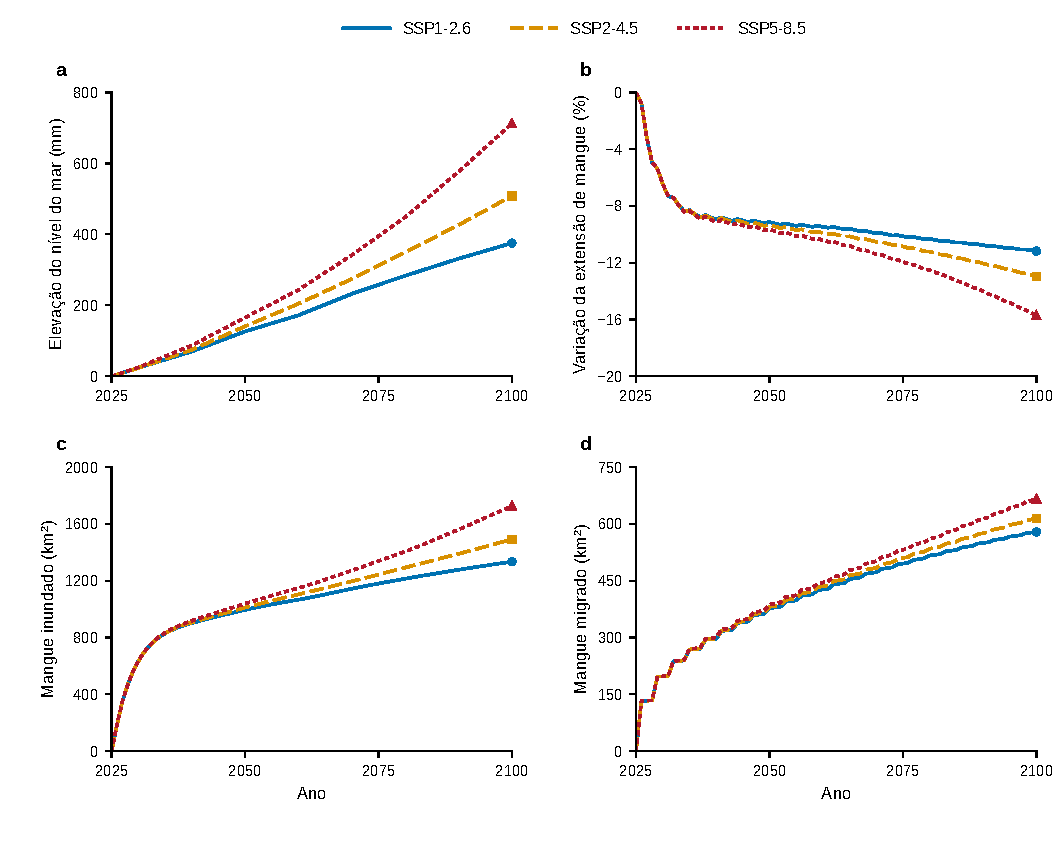
\includegraphics[width=\linewidth]{figuras/figura_2.pdf}
\caption{Trajetórias e evolução simulada dos manguezais entre 2025 e 2100. (a) Elevação acumulada do nível do mar; (b) variação relativa da extensão; (c) mangue de 2025 convertido em inundado; (d) mangue migrado. Cada curva representa uma execução, com parâmetros comuns e sem intervalos de incerteza.}
\label{fig:trajetorias}
\ifdefined\VersaoCega
\fonte{Fontes: trajetórias processadas de Garner et al. (2021) e saídas do modelo.}
\else
\fonte{Fontes: trajetórias processadas de Garner et al.\ (2021) e saídas conferidas do BR-MANGUE Studio 1.4.4.}
\fi
\end{figure}

Em 2050, a extensão simulada é de 6.141,9 km$^2$ no SSP1-2.6, 6.128,8 km$^2$ no SSP2-4.5 e 6.107,3 km$^2$ no SSP5-8.5. Em 2100, os valores diminuem para 6.003,2, 5.881,8 e 5.697,4 km$^2$, respectivamente (Tabela~\ref{tab:balanco}). As reduções líquidas correspondem a 755,7, 877,0 e 1.061,5 km$^2$, ou 11,18\%, 12,98\% e 15,70\% da cobertura simulável inicial. A diferença de extensão final entre os cenários extremos é de 305,8 km$^2$.

\begin{table}[htbp]
\centering
\caption{Balanço dos manguezais em 2100. Áreas em km$^2$, salvo a última linha.}
\label{tab:balanco}
\small
\begin{tabularx}{\linewidth}{Xrrr}
\toprule
Indicador & SSP1-2.6 & SSP2-4.5 & SSP5-8.5\\
\midrule
Mangue remanescente & 5.424,2 & 5.267,1 & 5.031,4\\
Mangue migrado & 579,0 & 614,7 & 666,0\\
Mangue inundado & 1.334,6 & 1.491,8 & 1.727,5\\
Extensão final & 6.003,2 & 5.881,8 & 5.697,4\\
Variação líquida & $-$755,7 & $-$877,0 & $-$1.061,5\\
Variação relativa (\%) & $-$11,18 & $-$12,98 & $-$15,70\\
\bottomrule
\end{tabularx}
\fonte{Fonte: saídas conferidas das três simulações.}
\end{table}

A migração compensa 43,38\%, 41,21\% e 38,55\% da área inundada em SSP1-2.6, SSP2-4.5 e SSP5-8.5, respectivamente. A maior expansão no SSP5-8.5 coincide, portanto, com menor compensação proporcional e maior perda líquida.

O primeiro passo produz 182,45 km$^2$ de mangue inundado nos três cenários e aproximadamente 132,7 km$^2$ de mangue migrado. Esse comportamento comum antecede a maior diferenciação das trajetórias e revela a influência da condição inicial e das regras locais sobre a resposta de curto prazo. Ao final do período, as curvas se separam tanto na perda da cobertura de 2025 como na expansão do estado migrado (Figura~\ref{fig:trajetorias}).

\subsection{Desempenho computacional}
Cada cenário processou 77.061.011 células válidas em 75 passos anuais, totalizando 5.779.575.825 operações de atualização célula-ano por execução e 17.338.727.475 nas três execuções. Essa contagem corresponde à visita e atualização de cada célula válida em cada passo; não representa apenas células cuja classe mudou. Os tempos foram de 6 h 37 min 49 s, 6 h 45 min 58 s e 6 h 48 min 20 s, respectivamente. A taxa média observada variou entre 235.896 e 242.134 operações por segundo, incluindo a gravação anual dos rasters (Tabela~\ref{tab:desempenho}). O pico de memória residente ficou entre 9,00 e 9,13 GiB.

\begin{table}[htbp]
\centering
\caption{Desempenho observado nas simulações da CMMA.}
\label{tab:desempenho}
\small
\begin{tabular}{lrrrr}
\toprule
Cenário & Tempo & Operações ($10^9$) & Operações s$^{-1}$ ($10^3$) & Pico RAM (GiB)\\
\midrule
SSP1-2.6 & 6:37:49 & 5,780 & 242,1 & 9,03\\
SSP2-4.5 & 6:45:58 & 5,780 & 237,3 & 9,00\\
SSP5-8.5 & 6:48:20 & 5,780 & 235,9 & 9,13\\
\bottomrule
\end{tabular}
\fonte{Fonte: metadados das execuções. O tempo inclui as atualizações anuais e a gravação dos rasters, sem o carregamento inicial dos dados nem a geração posterior de figuras e relatórios.}
\end{table}

\subsection{Distribuição espacial e coberturas de origem da migração}
Os mapas mostram remanescentes intercalados com áreas inundadas e células migradas nas bordas das coberturas naturais elegíveis (Figura~\ref{fig:espacial}). A ampliação comum evidencia maior extensão das alterações no SSP5-8.5.

\begin{figure}[htbp]
\centering
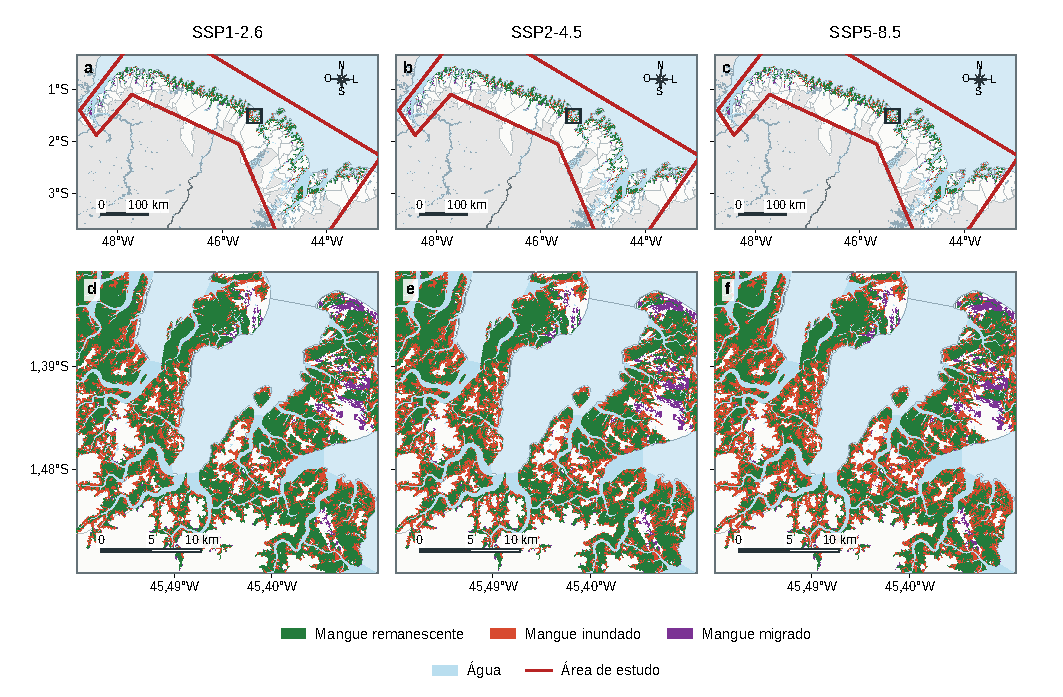
\includegraphics[width=\linewidth]{figuras/figura_3.pdf}
\caption{Estados dos manguezais em 2100. (a--c) Recorte regional nos três cenários. (d--f) Mesma janela de 30 $\times$ 30 km, indicada nos painéis superiores, selecionada por sua alta concentração de mudanças. Mangue remanescente e inundado referem-se à cobertura inicial de 2025. As cores indicam classes de estado, com resolução de origem de 30 m.}
\label{fig:espacial}
\fonte{Fontes: saídas do modelo; IBGE MMD 2025 e BC250, versão 2025. Projeção SIRGAS 2000 / Brazil Albers.}
\end{figure}

As florestas alagáveis representam 58,40\%, 58,38\% e 58,37\% do mangue migrado nos cenários SSP1-2.6, SSP2-4.5 e SSP5-8.5, respectivamente. Suas áreas convertidas aumentam de 338,14 para 388,79 km$^2$ entre os cenários extremos. A formação florestal responde por 21,19--21,99\%, e o campo alagado e área pantanosa por 13,73--15,03\%. Formação savânica, formação campestre e restinga herbácea ou arbustiva completam a distribuição (Material Suplementar S1, Figura S1).

Considerando a área inicial de cada categoria, a fração de floresta alagável convertida em mangue migrado varia de 6,51\% a 7,49\%. Para formação florestal, varia de 0,46\% a 0,55\%. Essa diferença mostra que a participação na migração total e a proporção de conversão de uma categoria descrevem aspectos distintos. Não se registra migração proveniente das classes antropizadas ou bloqueadas, conforme a restrição imposta pelo mapeamento de entrada.

\section{Discussão}
\subsection{Perda da cobertura inicial e acomodação continental}
Os três cenários produzem redução líquida de manguezais, acompanhada por aumento da área migrada. A direção dessas duas respostas é compatível com a coexistência de perda nas áreas expostas e estabelecimento em ambientes adjacentes descrita na literatura, embora as magnitudes dependam da formulação do modelo e das condições locais \citep{schuerch2018,woodroffe2016}. Na aplicação, a expansão compensa menos da metade da inundação acumulada da cobertura inicial. A diminuição dessa compensação entre SSP1-2.6 e SSP5-8.5 indica que a abertura de áreas elegíveis à migração não acompanha integralmente a perda calculada sob a maior forçante.

A predominância das florestas alagáveis relaciona a migração à configuração das coberturas adjacentes de 2025. O estabelecimento depende ainda de salinidade, dispersão e substrato, heterogêneos na costa amazônica \citep{menezes2008}. As transições identificam áreas prioritárias para investigação dessas condições.

A configuração mantém os usos de 2025, sem simular urbanização, abandono ou restauração. Essa restrição atua sobre pressões humanas espacialmente heterogêneas na costa amazônica \citep{hayashi2019}. O bloqueio de apicuns também exclui uma via de expansão documentada regionalmente \citep{menezes2008}. A migração calculada corresponde, assim, ao espaço permitido pelo agrupamento de classes.

\subsection{Relação com estudos anteriores da CMMA}
Tomaz et al.\ \citeyearpar{tomaz2019} delimitam a aplicação à porção maranhense da CMMA, identificada como Reentrâncias Maranhenses (seção de área de estudo e Figura 1). Nesse recorte, estimam expansão líquida de 7,2\% entre 2010 e 2100 com taxa constante de 3,18 mm ano$^{-1}$. O presente estudo abrange setores do Pará e Maranhão e utiliza outras condições iniciais, bases altimétricas, regras e forçantes. A diferença de sinal entre os balanços não constitui uma comparação controlada: envolve domínios espaciais distintos, além de diferenças metodológicas. Não se pode atribuí-la isoladamente ao cenário climático ou à versão do modelo.

Mapeamentos anteriores documentam a reorganização dos manguezais amazônicos \citep{cohen2003,cohen2018,nascimento2013,souzafilho2005}, mas suas datas, sensores e classificações impedem comparação direta dos totais com 2025. A aplicação compara três trajetórias com dados atualizados e contabiliza separadamente permanência, inundação e migração.

\subsection{Condicionantes da interpretação}
A referência vertical e a acurácia altimétrica influenciam diretamente a comparação entre a superfície e os níveis utilizados no modelo. O ANADEM reduz o viés de vegetação do Copernicus, mas sua avaliação continental ainda apresenta erros métricos \citep{laipelt2024}. Essas estatísticas não são uma validação local da CMMA, e as diferenças submétricas entre as trajetórias não asseguram precisão equivalente na localização de cada transição. A transferência da referência média de Itaqui, a concentração espacial de estações e o uso de máximas previstas de um único ano acrescentam incerteza ao parâmetro de 3,01 m. O desenho comum aos cenários permite comparação sob a mesma aproximação, sem eliminar seus efeitos sobre as áreas absolutas.

A uniformização da acreção reduz a heterogeneidade documentada nos testemunhos amazônicos \citep{lacerda2024,passos2023}. A taxa entra como acréscimo fixo à variável de elevação, inclusive no mangue inundado, enquanto a resposta real da superfície envolve aporte mineral, matéria orgânica e processos subsuperficiais \citep{woodroffe2016}. Da mesma forma, a idade funcional de três anos é uma parametrização de estabelecimento e propagação, cuja adequação espacial não foi estimada com observações locais de recrutamento. Os resultados avaliam esse conjunto de parâmetros; não quantificam a resposta a outras taxas de acreção ou idades de maturação.

As regras de transição também delimitam a interpretação. A propagação da inundação utiliza diferenças locais de elevação, e a classe água inclui corpos continentais sem diferenciação hidrodinâmica. A resposta inicial comum aos cenários, com 182,45 km$^2$ de mangue inundado no primeiro passo, indica um ajuste do estado de entrada às regras que não pode ser atribuído integralmente ao incremento climático de um ano. Não há execução de controle com nível constante para separar essa parcela. Por sua vez, a ausência de inundação posterior do mangue migrado favorece sua permanência no balanço e pode elevar a compensação calculada em relação a uma implementação com perda desses novos estados.

As trajetórias centrais não quantificam incertezas de projeção, parâmetros ou cartografia. A consistência computacional foi conferida; a capacidade preditiva requer validação ecológica independente \citep{olofsson2014}.

\section{Conclusões}
O estudo aplica três trajetórias regionais do IPCC ao recorte contínuo da CMMA entre Pará e Maranhão, ampliando a escala espacial de simulações anteriores concentradas no setor maranhense. Até 2100, as simulações indicam redução líquida de 11,18\% a 15,70\% da extensão de manguezais, com maior perda no SSP5-8.5. A migração compensa 38,55--43,38\% da inundação da cobertura inicial e ocorre predominantemente sobre florestas alagáveis. A contribuição inclui o balanço espacial por cenário, a origem das áreas migradas e o inventário de manguezais por município. O desempenho registrado demonstra que as três trajetórias puderam ser processadas em grade com 77,1 milhões de células válidas, com gravação anual dos mapas. Esses resultados fornecem informação espacial para o planejamento de adaptação climática e conservação costeira, em diálogo com as metas 13.1, 13.2, 14.2 e 15.1 dos ODS e com o eixo Meio Ambiente Valorizado e Resiliente do Plano Maranhão 2050 \citep{unitednations2015,maranhao2050}. As projeções permanecem condicionadas pela referência aproximada de maré, acreção uniforme, bloqueio de apicuns e permanência do mangue migrado; a capacidade preditiva requer validação ecológica independente.

\section*{Agradecimentos}
\ifdefined\VersaoCega
Agradecimentos e informações de financiamento omitidos para avaliação cega.
\else
O presente trabalho foi realizado com apoio da Coordenação de Aperfeiçoamento de Pessoal de Nível Superior -- Brasil (CAPES) -- Código de Financiamento 001. Os autores agradecem ao Laboratório de Geotecnologias e Ciências Ambientais (GEOTAM-UFMA).
\fi

\section*{Disponibilidade de dados e código}
\ifdefined\VersaoCega
Os identificadores persistentes e endereços de código e dados foram omitidos nesta cópia para avaliação cega. O conjunto de dados é identificado por referência anonimizada \citep{dados2026}; o Material Suplementar S1 documenta classes, trajetórias, cálculos e séries anuais.
\else
O BR-MANGUE Studio 1.4.4 está arquivado no Zenodo (DOI \url{https://doi.org/10.5281/zenodo.23527116}). O conjunto municipal de manguezais e o método de contagem estão no repositório do projeto, em \texttt{cmma\_municipalities\_2025} \citep{dados2026}. O Material Suplementar S1 (PDF), a Planilha Suplementar S1 e os arquivos tabulares associados estão disponíveis no repositório público do projeto: \url{https://github.com/oceanpep/br-mangue-studio/tree/main/docs/publications/oe2}.
\fi

\FloatBarrier
\begin{thebibliography}{99}
\interlinepenalty=10000
\bibitem[Allen(2002)]{allen2002}
ALLEN, J. A. Rhizophora mangle L. In: VOZZO, J. A. (ed.). \textbf{Tropical tree seed manual}. Washington, DC: USDA Forest Service, 2002. p. 690--692. Disponível em: \url{https://www.fs.usda.gov/psw/publications/allen/psw_2002_allen009.pdf}.

\ifdefined\VersaoCega
\bibitem[Estudo anterior(2014)]{bezerra2014}
REFERÊNCIA ANONIMIZADA. Estudo de autômatos celulares em manguezais da Ilha do Maranhão, 2014. Dados bibliográficos omitidos durante a avaliação cega.
\else
\bibitem[Bezerra et~al.(2014)]{bezerra2014}
BEZERRA, D. da S. et al. Simulating sea-level rise impacts on mangrove ecosystem adjacent to anthropic areas: the case of Maranhão Island, Brazilian Northeast. \textbf{Pan-American Journal of Aquatic Sciences}, v. 9, n. 3, p. 188--198, 2014. Disponível em: \url{https://panamjas.org/pdf_artigos/PANAMJAS_9%283%29_188-198.pdf}.
\fi

\bibitem[Centro de Hidrografia da Marinha(2001)]{chm2001}
CENTRO DE HIDROGRAFIA DA MARINHA. \textbf{Ficha F-21: RN2, Porto de Itaqui}. Levantamento GNSS, 2001. Disponível em: \url{https://www.marinha.mil.br/chm/sites/www.marinha.mil.br.chm/files/anexo_topogeodesico/f-21-413-009-2001.pdf}.

\bibitem[Centro de Hidrografia da Marinha(2018)]{chm2018}
CENTRO DE HIDROGRAFIA DA MARINHA. \textbf{Ficha F-41: Porto de Itaqui, estação 30110}. 2018. Disponível em: \url{https://www.marinha.mil.br/chm/sites/www.marinha.mil.br.chm/files/dados_de_mare/30110_-_porto_de_itaqui_f-41_-_tabuas_padrao_v1-18.pdf}.

\bibitem[Centro de Hidrografia da Marinha(2026)]{chm2026}
CENTRO DE HIDROGRAFIA DA MARINHA. \textbf{Tábuas das Marés 2026}. Niterói: Marinha do Brasil, 2026. Disponível em: \url{https://www.marinha.mil.br/chm/tabuas-de-mare-6?page=0}.

\bibitem[Cohen et~al.(2018)]{cohen2018}
COHEN, M. C. L. et al. Decadal-scale dynamics of an Amazonian mangrove caused by climate and sea level changes: inferences from spatial-temporal analysis and digital elevation models. \textbf{Earth Surface Processes and Landforms}, v. 43, p. 2876--2888, 2018. DOI: \url{https://doi.org/10.1002/esp.4440}.

\bibitem[Cohen \& Lara(2003)]{cohen2003}
COHEN, M. C. L.; LARA, R. J. Temporal changes of mangrove vegetation boundaries in Amazônia: application of GIS and remote sensing techniques. \textbf{Wetlands Ecology and Management}, v. 11, p. 223--231, 2003. DOI: \url{https://doi.org/10.1023/A:1025007331075}.

\bibitem[Dangremond \& Feller(2016)]{dangremond2016}
DANGREMOND, E. M.; FELLER, I. C. Precocious reproduction increases at the leading edge of a mangrove range expansion. \textbf{Ecology and Evolution}, v. 6, p. 5087--5092, 2016. DOI: \url{https://doi.org/10.1002/ece3.2270}.

\bibitem[Engelen et~al.(1995)]{engelen1995}
ENGELEN, G.; WHITE, R.; ULJEE, I.; DRAZAN, P. Using cellular automata for integrated modelling of socio-environmental systems. \textbf{Environmental Monitoring and Assessment}, v. 34, n. 2, p. 203--214, 1995. DOI: \url{https://doi.org/10.1007/BF00546036}.

\bibitem[Fox-Kemper et~al.(2021)]{fox2021}
FOX-KEMPER, B. et al. Ocean, cryosphere and sea level change. In: MASSON-DELMOTTE, V. et al. (ed.). \textbf{Climate Change 2021: The Physical Science Basis}. Cambridge: Cambridge University Press, 2021. p. 1211--1362. DOI: \url{https://doi.org/10.1017/9781009157896.011}.

\bibitem[Garner et~al.(2021)]{garner2021}
GARNER, G. G. et al. \textbf{IPCC AR6 Sea Level Projections}. Versão 20210809. Zenodo, 2021. Conjunto de dados. DOI: \url{https://doi.org/10.5281/zenodo.6382554}.

\bibitem[Gilman et~al.(2008)]{gilman2008}
GILMAN, E. L.; ELLISON, J.; DUKE, N. C.; FIELD, C. Threats to mangroves from climate change and adaptation options: a review. \textbf{Aquatic Botany}, v. 89, n. 2, p. 237--250, 2008. DOI: \url{https://doi.org/10.1016/j.aquabot.2007.12.009}.

\bibitem[Gorelick et~al.(2017)]{gorelick2017}
GORELICK, N. et al. Google Earth Engine: planetary-scale geospatial analysis for everyone. \textbf{Remote Sensing of Environment}, v. 202, p. 18--27, 2017. DOI: \url{https://doi.org/10.1016/j.rse.2017.06.031}.

\bibitem[Hayashi et~al.(2019)]{hayashi2019}
HAYASHI, S. N. et al. The effect of anthropogenic drivers on spatial patterns of mangrove land use on the Amazon coast. \textbf{PLOS ONE}, v. 14, n. 6, e0217754, 2019. DOI: \url{https://doi.org/10.1371/journal.pone.0217754}.

\bibitem[IBGE(2025a)]{ibge2025}
IBGE. \textbf{Malha Municipal Digital 2025: Pará e Maranhão}. Rio de Janeiro: IBGE, 2025a. Disponível em: \url{https://geoftp.ibge.gov.br/organizacao_do_territorio/malhas_territoriais/malhas_municipais/municipio_2025/UFs/}.

\bibitem[IBGE(2025b)]{ibgebc}
IBGE. \textbf{Base Cartográfica Contínua do Brasil, escala 1:250.000}. Versão 2025. Rio de Janeiro: IBGE, 2025b. Disponível em: \url{https://geoftp.ibge.gov.br/cartas_e_mapas/bases_cartograficas_continuas/bc250/versao2025/}.

\bibitem[Karney(s.d.)]{karney}
KARNEY, C. F. F. \textbf{GeographicLib: GeoidEval}. Documentação do cálculo de alturas geoidais. [S. l.], [s. d.]. Disponível em: \url{https://geographiclib.sourceforge.io/html/GeoidEval.1.html}.

\bibitem[Kauffman et~al.(2018)]{kauffman2018}
KAUFFMAN, J. B. et al. Carbon stocks of mangroves and salt marshes of the Amazon region, Brazil. \textbf{Biology Letters}, v. 14, 20180208, 2018. DOI: \url{https://doi.org/10.1098/rsbl.2018.0208}.

\bibitem[Kopp et~al.(2023)]{kopp2023}
KOPP, R. E. et al. The Framework for Assessing Changes To Sea-level (FACTS) v1.0: a platform for characterizing parametric and structural uncertainty in future global, relative, and extreme sea-level change. \textbf{Geoscientific Model Development}, v. 16, p. 7461--7489, 2023. DOI: \url{https://doi.org/10.5194/gmd-16-7461-2023}.

\bibitem[Lacerda et~al.(2024)]{lacerda2024}
LACERDA, L. D. de; FERREIRA, A. C.; BORGES, R.; WARD, R. Challenges to mangroves of the Semiarid Equatorial Coast of Brazil in the Anthropocene. \textbf{Cambridge Prisms: Coastal Futures}, v. 2, e17, 2024. DOI: \url{https://doi.org/10.1017/cft.2024.16}.

\bibitem[Laipelt et~al.(2024)]{laipelt2024}
LAIPELT, L. et al. ANADEM: a digital terrain model for South America. \textbf{Remote Sensing}, v. 16, n. 13, 2321, 2024. DOI: \url{https://doi.org/10.3390/rs16132321}.

\bibitem[Lee et~al.(2014)]{lee2014}
LEE, S. Y. et al. Ecological role and services of tropical mangrove ecosystems: a reassessment. \textbf{Global Ecology and Biogeography}, v. 23, p. 726--743, 2014. DOI: \url{https://doi.org/10.1111/geb.12155}.

\bibitem[Lovelock et~al.(2015)]{lovelock2015}
LOVELOCK, C. E. et al. The vulnerability of Indo-Pacific mangrove forests to sea-level rise. \textbf{Nature}, v. 526, p. 559--563, 2015. DOI: \url{https://doi.org/10.1038/nature15538}.

\bibitem[MapBiomas(2026a)]{mapbiomas2026}
MAPBIOMAS. \textbf{Coleção 11: cobertura e uso da terra, 30 m, 1985--2025}. MapBiomas Brasil, 2026. Disponível em: \url{https://brasil.mapbiomas.org/iniciativas-e-produtos/cobertura-e-uso-da-terra/cobertura-30m/cobertura/}.

\bibitem[MapBiomas(2026b)]{mapbiomasareas2026}
MAPBIOMAS. \textbf{Coleção 11: área de cobertura e uso da terra por estado, 1985--2025}. MapBiomas Brasil, 2026. Planilha de estatísticas, classe Mangue, ano 2025. Disponível em: \url{https://brasil.mapbiomas.org/wp-content/uploads/sites/3/2026/08/MAPBIOMAS_BRAZIL-COL.11-BIOME_STATE.xlsx}.

\bibitem[Maranhão(2024)]{maranhao2050}
MARANHÃO (Estado). Secretaria de Estado do Planejamento e Orçamento. \textbf{Plano Estratégico de Longo Prazo Maranhão 2050}. São Luís: SEPLAN-MA, 2024. Disponível em: \url{https://data.seplan.ma.gov.br/PLANO_MARANHAO_2050.pdf}.

\bibitem[Menezes et~al.(2008)]{menezes2008}
MENEZES, M. P. M. de; BERGER, U.; MEHLIG, U. Mangrove vegetation in Amazonia: a review of studies from the coast of Pará and Maranhão States, north Brazil. \textbf{Acta Amazonica}, v. 38, n. 3, p. 403--420, 2008. DOI: \url{https://doi.org/10.1590/S0044-59672008000300004}.

\bibitem[Nascimento Jr. et~al.(2013)]{nascimento2013}
NASCIMENTO JR., W. R. et al. Mapping changes in the largest continuous Amazonian mangrove belt using object-based classification of multisensor satellite imagery. \textbf{Estuarine, Coastal and Shelf Science}, v. 117, p. 83--93, 2013. DOI: \url{https://doi.org/10.1016/j.ecss.2012.10.005}.

\bibitem[Natural Earth(2022)]{naturalearth}
NATURAL EARTH. \textbf{Admin 0 -- Countries}. Versão 5.1.1. 2022. Dados cartográficos. Disponível em: \url{https://github.com/nvkelso/natural-earth-vector/tree/v5.1.1}.

\bibitem[Olofsson et~al.(2014)]{olofsson2014}
OLOFSSON, P. et al. Good practices for estimating area and assessing accuracy of land change. \textbf{Remote Sensing of Environment}, v. 148, p. 42--57, 2014. DOI: \url{https://doi.org/10.1016/j.rse.2014.02.015}.

\bibitem[OpenTopography(2025)]{anadem2025}
OPENTOPOGRAPHY. \textbf{ANADEM: a digital terrain model for South America}. 2025. Metadados do conjunto de dados. DOI: \url{https://doi.org/10.5069/G9736P4G}.

\bibitem[Passos et~al.(2023)]{passos2023}
PASSOS, T. et al. Low carbon accumulation in a macro-tidal mangrove forest on the Amazon coast. \textbf{Limnology and Oceanography}, v. 68, p. 1936--1948, 2023. DOI: \url{https://doi.org/10.1002/lno.12396}.

\bibitem[Saintilan et~al.(2020)]{saintilan2020}
SAINTILAN, N.; KHAN, N. S.; ASHE, E.; KELLEWAY, J. J.; ROGERS, K.; WOODROFFE, C. D.; HORTON, B. P. Thresholds of mangrove survival under rapid sea level rise. \textbf{Science}, v. 368, n. 6495, p. 1118--1121, 2020. DOI: \url{https://doi.org/10.1126/science.aba2656}.

\bibitem[Schuerch et~al.(2018)]{schuerch2018}
SCHUERCH, M. et al. Future response of global coastal wetlands to sea-level rise. \textbf{Nature}, v. 561, p. 231--234, 2018. DOI: \url{https://doi.org/10.1038/s41586-018-0476-5}.

\ifdefined\VersaoCega
\bibitem[Software do estudo(2026a)]{studio2026}
SOFTWARE DO ESTUDO. Implementação de autômato celular, versão 1.4.4. Dados bibliográficos e identificador suprimidos para avaliação cega.
\else
\bibitem[Sousa et~al.(2026a)]{studio2026}
SOUSA, F. M.; BEZERRA, D. da S.; COSTA, S. S.; SANTOS, R. L. \textbf{BR-MANGUE Studio}. Versão 1.4.4. Zenodo, 2026a. Software. DOI: \url{https://doi.org/10.5281/zenodo.23527116}.
\fi

\ifdefined\VersaoCega
\bibitem[Conjunto de dados do estudo(2026b)]{dados2026}
CONJUNTO DE DADOS DO ESTUDO. Inventário municipal de manguezais, 2025. Dados bibliográficos e endereço suprimidos para avaliação cega.
\else
\bibitem[Sousa et~al.(2026b)]{dados2026}
SOUSA, F. M.; BEZERRA, D. da S.; COSTA, S. S.; SANTOS, R. L. \textbf{Manguezais da CMMA por município -- 2025}. Versão a1a9aea. GitHub, 2026b. Conjunto de dados. Disponível em: \url{https://github.com/oceanpep/br-mangue-studio/tree/a1a9aea6a176e0bb177f088f8be3ec5932248e4d/datasets/cmma_municipalities_2025}.
\fi

\bibitem[Souza Jr. et~al.(2020)]{souzajr2020}
SOUZA JR., C. M. et al. Reconstructing three decades of land use and land cover changes in Brazilian biomes with Landsat archive and Earth Engine. \textbf{Remote Sensing}, v. 12, n. 17, 2735, 2020. DOI: \url{https://doi.org/10.3390/rs12172735}.

\bibitem[Souza-Filho(2005)]{souzafilho2005}
SOUZA-FILHO, P. W. M. Costa de manguezais de macromaré da Amazônia: cenários morfológicos, mapeamento e quantificação de áreas usando dados de sensores remotos. \textbf{Revista Brasileira de Geofísica}, v. 23, n. 4, p. 427--435, 2005. DOI: \url{https://doi.org/10.1590/S0102-261X2005000400006}.

\bibitem[Tomaz et~al.(2019)]{tomaz2019}
TOMAZ, R. B. et al. Predicting the impacts of sea-level rise on the Amazon Macrotidal Mangrove Coast. \textbf{Revista Brasileira de Climatologia}, v. 25, p. 15--34, 2019. DOI: \url{https://doi.org/10.5380/abclima.v25i0.60891}.

\bibitem[United Nations(2015)]{unitednations2015}
UNITED NATIONS. \textbf{Transforming our world: the 2030 Agenda for Sustainable Development}. A/RES/70/1. New York: United Nations, 2015. Disponível em: \url{https://sdgs.un.org/2030agenda}.

\bibitem[Woodroffe et~al.(2016)]{woodroffe2016}
WOODROFFE, C. D. et al. Mangrove sedimentation and response to relative sea-level rise. \textbf{Annual Review of Marine Science}, v. 8, p. 243--266, 2016. DOI: \url{https://doi.org/10.1146/annurev-marine-122414-034025}.

\bibitem[Xie et~al.(2022)]{xie2022}
XIE, D. et al. Implications of coastal conditions and sea-level rise on mangrove vulnerability: a bio-morphodynamic modeling study. \textbf{Journal of Geophysical Research: Earth Surface}, v. 127, e2021JF006301, 2022. DOI: \url{https://doi.org/10.1029/2021JF006301}.
\end{thebibliography}
\end{document}
